\documentclass{article} 
\usepackage{times}
\usepackage{amsmath}
\usepackage{hyperref}
\usepackage{graphicx}
\usepackage{tikz}
\usetikzlibrary{bayesnet}

% notation for transition probabilities     
\newcommand{\TGluToGlu}{\theta_{\mathsf{Glu}\rightarrow\mathsf{Glu}}}
\newcommand{\TGalToGlu}{\theta_{\mathsf{Gal}\rightarrow\mathsf{Glu}}}

% notation for growth rates under different nutrients
% glucose
\newcommand{\GluRate}{\mu_{\mathsf{Glu}}}
% galactose
\newcommand{\GalRate}{\mu_{\mathsf{Gal}}}
% maltose
\newcommand{\MalRate}{\mu_{\mathsf{Mal}}}
% growth rate where the cell is mismatched to environment
\newcommand{\MisRate}{\mu_{\mathsf{Mis}}}


% notation for probability distributions
\newcommand{\Poi}{\mathrm{Poisson}}
\newcommand{\Norm}{\mathrm{Normal}}
\newcommand{\Dir}{\mathrm{Dirichlet}}
\newcommand{\Mult}{\mathrm{Multinomial}}

% integral notation
\newcommand*\diff{\mathop{}\!\mathrm{d}}

\begin{document}

%%
%% To edit TeX generated figures in Illustrator,
%% copy the fonts first to Illustrator
%%
% cp /usr/local/texlive/2015/texmf-dist/fonts/type1/public/amsfonts/cm/* ~/Library/Application\ Support/Adobe/Fonts/
% cp /usr/local/texlive/2015/texmf-dist/fonts/type1/public/amsfonts/symbols/* ~/Library/Application\ Support/Adobe/Fonts/

\begin{figure}[t]
\centering
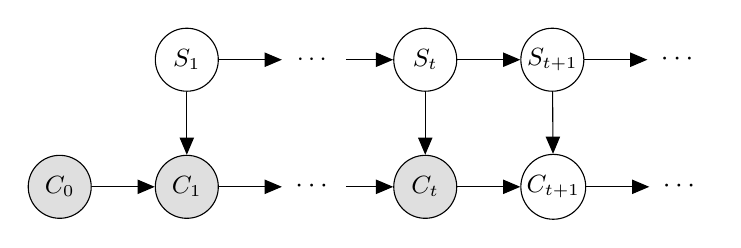
\begin{tikzpicture}
  % Define nodes
  \node[latent, minimum size=0.8cm] (s1) {{\small $S_{1}$}};
  \node[const, minimum size=0.8cm, right=0.8cm of s1] (sdots1) {{\small $\cdots$}};
  \node[latent, minimum size=0.8cm, right=0.1cm of sdots1, xshift=0.5cm] (sT) {{\small $S_{t}$}};
  \node[latent, minimum size=0.8cm, right=0.8cm of sT] (sTplusone) {{\small $S_{t+1}$}};
  \node[const, minimum size=0.8cm, right=0.8cm of sTplusone] (sdots2) {$\cdots$};
  \node[obs, minimum size=0.8cm, below=2cm of s1, yshift=1.2cm] (c1) {{\small $C_{1}$}};
  \node[const, minimum size=0.8cm, right=0.8cm of c1] (cdots1) {$\cdots$};
  \node[obs, minimum size=0.8cm, below=2cm of sT, yshift=1.2cm] (cT) {{\small $C_{t}$}};
  \node[latent, minimum size=0.8cm, right=0.8cm of cT] (cTplusone) {{\small $C_{t+1}$}};
  \node[const, minimum size=0.8cm, right=0.8cm of cTplusone] (cdots2) {$\cdots$};
  % initial carbon state
  \node[obs, minimum size=0.8cm, left=0.8cm of c1] (c0) {{\small $C_{0}$}}; 
  % connect switch states to each other
  \edge {s1} {sdots1} ; 
  \edge {sdots1} {sT} ;
  \edge {sT} {sTplusone} ;
  \edge {sTplusone} {sdots2} ;
  % connect switch states to carbon source
  \edge {s1} {c1} ;
  \edge {sT} {cT} ;
  \edge {sTplusone} {cTplusone} ;
  % connect carbon sources to each other
  \edge {c0} {c1} ;
  \edge {c1} {cdots1} ;
  \edge {cdots1} {cT} ;
  \edge {cT} {cTplusone} ; 
  \edge {cTplusone} {cdots2} ;
\end{tikzpicture}
\caption{\textbf{Dynamic Bayesian model for meta-changing environments}. Shown in graphical model notation \cite{JordanGraphicalModels2004}: nutrients (grey nodes) are observed, switching states are hidden (white nodes). Nutrient value at time $t$, $C_{t}$, depends on the nutrient value at time $t-1$, $C_{t-1}$, and on the switch state $S_{t}$. See Figure \ref{suppfig:GraphicalModel} for detailed graphical model.}
\label{fig3}
\end{figure}
%
%
%\begin{figure}[t]
%\centering
%\begin{tikzpicture}
%  % Define nodes
%  \node[latent, minimum size=0.8cm] (s1) {{\small $S_{1}$}};
%  \node[latent, minimum size=0.8cm, right=0.8cm of s1] (s2) {{\small $S_{2}$}};
%  \node[const, minimum size=0.8cm, right=0.8cm of s2] (sdots1) {{\small $\cdots$}};
%  \node[latent, minimum size=0.8cm, right=0.1cm of sdots1, xshift=0.5cm] (sT) {{\small $S_{t}$}};
%  \node[latent, minimum size=0.8cm, right=0.8cm of sT] (sTplusone) {{\small $S_{t+1}$}};
%  \node[const, minimum size=0.8cm, right=0.8cm of sTplusone] (sdots2) {$\cdots$};
%  \node[obs, minimum size=0.8cm, below=2cm of s1, yshift=1.2cm] (c1) {{\small $C_{1}$}};
%  \node[obs, minimum size=0.8cm, below=2cm of s2, yshift=1.2cm] (c2) {{\small $C_{2}$}};
%  \node[const, minimum size=0.8cm, right=0.8cm of c2] (cdots1) {$\cdots$};
%  \node[obs, minimum size=0.8cm, below=2cm of sT, yshift=1.2cm] (cT) {{\small $C_{t}$}};
%  \node[latent, right=2cm of cT) (X) {x};
%%  \node[latent, below=2cm of c0) (X) {$X$};
%%  \node[latent, below=2cm of sTplusone) (cTplus1) {$X$};
%%  \node[const, minimum size=0.8cm, right=0.8cm of cTplus1] (cdots2) {$\cdots$};
%  % initial carbon state
%  \node[obs, minimum size=0.8cm, left=0.8cm of c1] (c0) {{\small $C_{0}$}}; 
%  % connect switch states to each other
%  \edge {s1} {s2} ; 
%  \edge {s2} {sdots1} ;
%  \edge {sdots1} {sT} ;
%  \edge {sT} {sTplusone} ;
%  \edge {sTplusone} {sdots2} ;
%  % connect switch states to carbon source
%  \edge {s1} {c1} ;
%  \edge {s2} {c2} ;
%  \edge {sT} {cT} ;
%  % connect carbon sources to each other
%  \edge {c0} {c1} ;
%  \edge {c1} {c2} ;
%  \edge {c2} {cdots1} ;
%  \edge {cdots1} {cT} ;
%%  \edge {cT} {cdots2} ;
%\end{tikzpicture}
%\caption{\textbf{Dynamic Bayesian model for meta-changing environments}. Shown in graphical model notation \cite{JordanGraphicalModels2004}: nutrients (grey nodes) are observed, switching states are hidden (white nodes). Nutrient value at time $t$, $C_{t}$, depends on the nutrient value at time $t-1$, $C_{t-1}$, and on the switch state $S_{t}$. See Figure \ref{suppfig:GraphicalModel} for detailed graphical model.}
%\label{fig3}
%\end{figure}


\end{document}